%%%% fatec-article.tex, 2024/03/10

%% Classe de documento
\documentclass[
  a4paper,%% Tamanho de papel: a4paper, letterpaper (^), etc.
  12pt,%% Tamanho de fonte: 10pt (^), 11pt, 12pt, etc.
  english,%% Idioma secundário (penúltimo) (>)
  brazilian,%% Idioma primário (último) (>)
]{article}

%% Pacotes utilizados
\usepackage[]{fatec-article}
\Author{1}{Name={Arthur Parra da Silva\\ Guilherme Shimada Pereira \\ Gustavo Pinto Kletelinger\\ João Vitor da Silva Rosa \\ Matheus Bertoldo de Oliveira}}

\Author{2}{Name={\{ arthur.silva100@fatec.sp.gov.br \}\\ \{ guilherme.pereira112@fatec.sp.gov.br \} \\ \{ gustavo.kletelinger@fatec.sp.gov.br\} \\ \{joao.rosa42@fatec.sp.gov.br\} \\ \{ matheus.oliveira256@fatec.sp.gov.br \}}}

%% Definição das palavras-chaves/keywords
\Keyword{1}{Pinta Preta dos Citros}{Citrus Black Spot}
\Keyword{2}{Visão Computacional}{Computational Vision}
\Keyword{3}{Agricultura de Precisão}{Precision Agriculture}

%%%% Resumo no idioma primário (brazilian)
\begin{Abstract}[brazilian]%% Idioma (brazilian ou english)
  O resumo FATEC Registro é uma descrição completa e concisa dos componentes-chave da metodologia do estudo e dos achados importantes da pesquisa. Normalmente, o resumo é o primeiro encontro do leitor com uma pesquisa ou relato, sendo algumas vezes o único elemento recuperado e/ou revisado nas bases de dados científicos. Esse elemento provê a primeira impressão, muitas vezes a mais importante, identificando o valor potencial ou a relevância do enfoque da pesquisa e dos resultados. Se o resumo for bem escrito, ele atrairá leitores para obter uma cópia do manuscrito completo que será incorporado aos que já foram encontrados, e seu trabalho será citado. Se o resumo for mal escrito, a pesquisa poderá ser ignorada ou, até mesmo, esquecida.
\end{Abstract}

%%%% Resumo no idioma secundário (english)
\begin{Abstract}[english]%% Idioma (brazilian ou english)
The summary is a complete and concise description of the key components of the study methodology and important research findings. Typically, the summary is the reader's first encounter with a research report or paper, and sometimes it is the only element retrieved and/or reviewed in scientific databases. This element provides the first impression, often the most important one, identifying the potential value or relevance of the research approach and findings. If the summary is well-written, it will attract readers to obtain a copy of the full manuscript that will be incorporated into those already found, and your work will be cited. If the summary is poorly written, the research may be ignored or even forgotten.
\end{Abstract}

%% Processamento de entradas (itens) do índice remissivo (makeindex)
\makeindex%

%% Arquivo(s) de referências
\addbibresource{fatec-article.bib}

%% Início do documento
\begin{document}

% Seções e subseções
%\section{Título de Seção Primária}%

%\subsection{Título de Seção Secundária}%

%\subsubsection{Título de Seção Terciária}%

%\paragraph{Título de seção quaternária}%

%\subparagraph{Título de seção quinária}%

\section*{Introdução}%
\label{sect:intro}
Os Objetivos de Desenvolvimento Sustentável (ODSs) foram adotados pela Organização das Nações Unidas \cite{ONU2025} no ano de 2015, estabelecendo parâmetros para políticas nacionais sobre 17 temáticas que impactam o desenvolvimento humano em todos os países, que devem alcançá-los até o ano de 2030, por meio da cooperação internacional. Entre esses objetivos, o projeto de identificação da pinta preta (\emph{Phyllosticta citricarpa}) por visão computacional relaciona-se profundamente com as ODSs 2, 9 e 12, que propõem medidas para garantir segurança alimentar com agricultura sustentável, fomento da inovação nos setores produtivos e eficiência no uso dos recursos naturais, respectivamente. Esses objetivos serão trabalhados com enfoque na tangerina ponkan (\emph{Citrus reticulata}), uma cultura de destaque na região do Vale do Ribeira que pode contrair uma diversidade de doenças e avarias com sintomas semelhantes aos da pinta preta.

Sendo o Brasil o maior produtor mundial de laranja e suco de laranja \cite{USDA2025}, torna-se evidente a importância nacional deste gênero de frutas, conhecidas como citros (\emph{Citrus}). Fazem parte deste gênero as espécies de laranja, limão, lima, tangerina/mexerica, pomelo/toranja e cidra. Dentre elas, a tangerina possui um grande valor socioeconômico no Vale do Ribeira, uma área histórica e com forte agricultura familiar localizada entre os estados de São Paulo e Paraná. Um levantamento da Secretaria de Agricultura e Abastecimento (SEAB) realizado em 2020 revelou que o Vale produziu mais de 98 mil toneladas de citros, das quais 94\% foram tangerinas e 92\% destas foram da variedade ponkan. Somente as tangerinas renderam um valor bruto de produção de aproximadamente 168,3 milhões de reais para toda a citricultura da região, sendo a parte paranaense responsável por cerca de 163,2 milhões de reais \cite{Parana2021}.

Como dito anteriormente, a agricultura familiar é um pilar fundamental na economia do Vale do Ribeira, uma vez que contribui para a geração de renda, segurança alimentar e preservação ambiental em municípios onde os índices de desenvolvimento humano (IDH) geralmente estão abaixo da média estadual. Nesse contexto, a tangerina ponkan se adaptou bem às condições locais, pois a drenagem do solo incentiva o crescimento de raízes profundas para melhor captação de água; já o clima subtropical úmido, com alta umidade relativa do ar e temperaturas moderadas a altas, favorece a suculência e o tamanho dos frutos \cite{Borges2021}.

Essas características de agrado do consumidor definem a tangerina como um produto de comercialização principalmente in-natura, abastecendo não apenas o mercado externo, mas toda uma cadeia de pequenas propriedades familiares que são afetadas diretamente pelos problemas da cultura. Por exemplo, a sazonalidade do mercado, em razão da safra concentrada entre os meses de abril e julho, pode afetar diretamente famílias que têm o cultivo de ponkan como fonte de renda principal. Outro fator decisivo é a produtividade, muitas vezes prejudicada por questões fitossanitárias, ou seja, pragas e doenças. 

O cenário nacional de citros enfrenta grandes ameaças de agentes nocivos como insetos, bactérias e fungos. Atualmente, o huanglongbing ou greening (HLB) é considerado a maior ameaça à cadeia citrícola, tendo em vista suas capacidades destrutivas e a ausência de medidas curativas \cite{rodrigues2016hlb}. A clorose variegada dos citros (CVC) é outra doença bacteriana relevante, a qual coloniza os vasos do xilema da planta e dificulta o transporte de nutrientes e água, reduzindo drasticamente a produtividade da lavoura \cite{Alves2003}. Já a pinta preta, segundo \textcite{SilvaJunior2016}, foi relatada em 1980 no estado do Rio de Janeiro e encontra-se praticamente em todas as regiões citrícolas do país. Trata-se de uma doença fúngica causada pelas variações de reprodução sexuada \emph{Phyllostictina citricarpa} e assexuada \emph{Guignardia citricarpa}. Caracteriza-se pela queda prematura dos frutos, cujas cascas são acometidas por lesões que também desqualificam significativamente o produto para comercialização. Por esse motivo, “o manejo da doença em pomares para o mercado interno deve ser muito rigoroso e eficiente” \cite{SilvaJunior2016}.

No entanto, o mesmo estudo aponta que os sintomas da pinta preta, principalmente as lesões, podem gerar confusão para o produtor. Isso acontece porque elas são dotadas de grande variabilidade e geralmente se assemelham a danos mecânicos ou insetos, com grandes chances da doença não ser detectada até que atinja com severidade a planta. Os principais sintomas são manchas dura, sardenta, virulenta, rendilhada, trincada e a falsa melanose, com manifestação favorecida pela exposição ao sol em altas temperaturas \cite{SilvaJunior2016}.

Quando observa-se a falta de treinamentos técnicos e a escassez tecnológica como realidade dominante na agricultura familiar, é possível inferir a ameaça que a pinta preta representa para a produção de tangerina ponkan no Vale do Ribeira. Outro agravante é o próprio clima local, que propicia as contaminações por fungos em razão das altas taxas de umidade e calor. Portanto, as medidas de prevenção também precisam ser desenvolvidas, visando evitar a disseminação do fungo pelos pomares e, consequentemente, diminuir os custos de controle. Dentre as práticas preventivas, destacam-se a inspeção da doença, controle de entrada de materiais e mudas certificadas, nutrição e sanidade do pomar e remoção dos frutos infectados antes da florada \cite{Fundecitrus2025}.

Para o propósito de otimizar os processos de prevenção da pinta preta na cultura da ponkan, este projeto pretende desenvolver uma ferramenta baseada em Visão Computacional, que decorre da evolução tecno-científica e, mais especificamente, da evolução dos algoritmos de Inteligência Artificial (IA). 

IA é compreendida como campo de estudo dos sistemas capazes de realizar tarefas propriamente humanas, nascida no período da Segunda Guerra Mundial e oficializada em 1956, com a reunião de cientistas na Conferência de Dartmouth \cite{coelho2012turing}. Desde então, a IA cresceu ao ponto de, atualmente, automatizar e integrar soluções em diversos setores da sociedade, desde geradores de texto e imagens até carros, robôs e drones autônomos. Já a Visão Computacional é uma área da IA que procura emular o funcionamento da visão humana a partir do processamento de imagens, segundo \textcite{marengoni2009opencv}. A partir de bases de dados satisfatórias, algoritmos de Visão Computacional podem ser alimentados com vídeos e imagens e treinados para reconhecer formas, objetos, padrões de cores e texturas.

Este projeto utilizará esses princípios para produzir um sistema de identificação da pinta preta para telefones celulares, de forma a servir como uma ferramenta fácil e rápida de pré-diagnóstico para produtor, que poderá tomar decisões mais assertivas e inserir agricultura de precisão no seu manejo.

\section*{OBJETIVO} \label{sect:obj}

Desenvolver um sistema capaz de identificar sintomas da pinta preta na tangerina ponkan, capturados em foto via câmera de telefone celular, utilizando métodos de Inteligência Artificial e Visão Computacional de modo a otimizar as medidas preventivas em campo. 

Em paralelo, o projeto possui objetivos secundários que complementam sua finalidade principal:\\


\begin{itemize}
    \item Satisfazer parâmetros de tempo de resposta do pré-diagnóstico menor que 5 minutos;
    \item Desenvolver modelos de visão computacional para processamento de imagem;
    \item Desenvolver modelos de redes neurais para análise e diferenciação de sintomas da pinta preta em relação a outras doenças semelhantes;
    \item Construir interfaces de software simples e intuitivas;
    \item Emitir recomendações de manejo personalizadas para o produtor, baseadas em dados climáticos; 
    \item Utilizar conjuntos de dados organizados e diversificados com sintomas da pinta preta para treinamento e teste em rede neural.
\end{itemize}


\section*{ESTADO DA ARTE} \label{sect:estadoarte}

Segundo Molin, Amaral e Colaço (2015), a agricultura de precisão (AP) é uma abordagem da agricultura que pode ser definida de várias formas, a depender do ponto de vista analisado. Em sua fase inicial, estava fortemente vinculada ao georreferenciamento (GPS) e, mais recentemente, pode ser entendida como a aplicação de Tecnologia da Informação (TI) durante a condução das lavouras. De qualquer maneira, a AP está fundamentada na compreensão de que as propriedades agrícolas não são uniformes espacialmente ou ao longo do tempo, o que exige o desenvolvimento de estratégias para gerenciar a heterogeneidade das lavouras e seus respectivos problemas.

Nesse contexto, o mercado nacional da AP já apresenta muitas soluções avançadas e diferentes, dentre as quais se destacam a ampla adoção de drones, tratores autônomos, sensores e serviços de monitoramento. Segundo a \textcite{ANAC2025}, entre 2023 e 2024 o número de cadastros de drones agrícolas saltou de 674 para 7.312, o que configura um aumento de mais de 10 vezes. Sensores multiespectrais, climáticos e de solo ajudam os produtores a acompanhar e ajustar processos como adubação e irrigação com bases de dados precisos, e quando integrados a plataformas digitais, entende-se como uso da Internet das Coisas (IOT) para reduzir desperdícios ao permitir monitoramento remoto das fazendas. Em relação a plataformas digitais para compra e venda, uma pesquisa realizada em 2020 pelo conjunto Embrapa, Sebrae e Inpe revelou que são utilizadas por pelo menos 40\% dos produtores. 

Nesse retrato,  a visão computacional “pode ser empregada na detecção de doenças e pragas, na estimação de safra e na avaliação não invasiva de atributos como qualidade, aparência e volume, além de ser componente essencial em sistemas robóticos agrícolas” \cite{santos2020visao}. O mesmo estudo aborda a classificação de padrões associados a objetos de interesse e sintomas de doenças e pragas como problemas  perceptuais abordados pela visão computacional, geralmente capturados em imagens por câmeras acopladas em tratores, robôs e drones. Cita também os problemas geométricos, advindos da perda de informações de profundidade em imagens bidimensionais e que podem ser recuperadas por algoritmos de visão computacional que interpretem múltiplas imagens de uma mesma cena.

Uma das soluções para detecção de doenças baseada na visão computacional e dedicada à citricultura é o trabalho de \cite{Pazoti2005}, que propôs o CITRUSVIS como sistema para auxiliar na identificação e contagem automática de ascósporos do fungo \emph{G. citricarpa}, causador da pinta preta, a fim de reduzir o tempo e os erros associados à análise manual. O fluxo de funcionamento inicia com a aquisição de imagens digitais de discos de coletas - são materiais acrílicos e adesivos onde se depositam os ascósporos e outras partículas sólidas sugadas por um equipamento chamado caça-esporo. Os discos são tingidos de corante láctico azul para melhor visualização e fotografados por microscópio por uma câmera digital de 640 x 512 \emph{pixels}. O pré-processamento das imagens incluiu a conversão para padrão HSI (matiz, saturação e intensidade) para contrastar e separar esporos corados do fundo branco; técnica de limiarização (\emph{thresholding}) que define cada \emph{pixel} como preto ou branco; filtros não lineares e operações morfológicas que suavizam os ruídos na imagem preservando as bordas dos esporos e a técnica transformada \emph{watershed}, que isola esporos colados ou sobrepostos. Após a extração das características de curvatura da forma e descritores de Fourier, a classificação usou um modelo de rede neural artificial (RNA) com aprendizado supervisionado, o qual recebeu 60 descritores de entrada que passaram por 2 camadas escondidas, com 20 e 15 neurônios. Como alternativa, testaram o classificador por método da distância mínima, que atribui a partícula à classe pelo vetor de características médias.
O protótipo foi integrado com uma interface gráfica no \emph{software} de cálculo numérico MATLAB. Com relação aos resultados, a RNA obteve 98\% de acurácia em amostras pré-selecionadas e 96,6\% em testes gerais, superando os 92\% do classificador por distância mínima; além disso, o tempo médio de processamento para cada imagem foi de 66 segundos. Concluiu-se um desempenho satisfatório na identificação dos ascósporos, podendo substituir parcialmente a análise manual dos especialistas, apesar de limitações na qualidade das imagens oriundas da fotografia em microscópio, como ruídos, sobreposição e baixa resolução.

Outro trabalho que utilizou redes neurais artificiais para processar imagens foi o de \cite{Ribeiro2012} que objetivou a diferenciação do \emph{greening} de outras doenças foliares e deficiências nutricionais em citros, uma vez que a identificação visual é falha e a Reação em Cadeia de Polimerase (PCR), técnica molecular para identificar DNA/RNA de organismos com alta precisão, é cara e demorada. Foram usadas amostras de 60 folhas de citros com sintomas de \emph{greening}, CVC, rubelose e deficiências de magnésio, manganês e zinco, cujas imagens foram digitalizadas em \emph{scanner} fotográfico. O pré-processamento baseou-se na segmentação das cores verdes, amarelas e marrons das manchas do \emph{greening} através de uma RNA treinada com 46 imagens, e as restantes de validação. Todo o treinamento foi feito por \emph{pixels} rotulados, que passaram por 3 camadas escondidas e ganharam máscaras binárias que definem as manchas. Foram extraídos descritores de forma ao aplicar cálculos matemáticos nas máscaras binárias, gerando uma quantidade de atributos que serão guardados em vetores e, depois, em quadrantes que medem a assimetria das manchas. A classificação das doenças também usou RNA e construiu escalas de severidade dos sintomas em diagrama. 
O estudo comentou desafios como a alta similaridade dos sintomas, a amostra reduzida de 60 folhas e o uso isolado da cor amarela, que não foi suficiente para discriminar o \emph{greening}. Ainda sim, a segmentação por cor com RNA obteve 96,04\% de precisão. No entanto, na classificação geral, considerando todas as doenças, os resultados variaram entre 43\% e 63\%. Concluiu-se que a RNA foi viável para auxiliar a diferenciação do \emph{greening} e pode ser usada para complementar a inspeção visual no campo, porém é necessário combinar a classificação de cores com os descritores de forma para alavancar a acurácia.

Um estudo mais próximo dos objetivos deste projeto e também recente foi o de \textcite{Momeny2022}, que se aprofundou no desenvolvimento de redes neurais convolucionais (CNNs) aliadas a uma estratégia chamada \emph{learning-to-augment}, que cria dados artificiais para treinamento do modelo na detecção da pinta preta (conhecida em inglês como \emph{Black Spot}) em laranjas. A base de dados (dataset) utilizada totalizou 1896 imagens de laranjas divididas em classes de frutos verdes, meia-maturação, maduros e com pinta preta - todas capturadas com \emph{smartphone} Samsung SM-J500H com câmera de 4128 x 2322 \emph{pixels}. Também foi utilizada uma versão do MATLAB como \emph{software} de processamento, e alguns modelos de \emph{deep learning} foram testados, como MobileNetV2, GoogleNet e DenseNet201. Os resultados demonstraram melhor desempenho do modelo ResNet50, que alcançou acurácia total de 99,5\% com 100\% de sensibilidade e especificidade, ou seja, sem desperceber frutos doentes nem confundir frutos saudáveis. 
 
Apesar dos dois primeiros artigos possuírem métodos de captura de imagens complexos ou demasiadamente manuais, ambos evidenciam o potencial das redes neurais artificiais e técnicas de processamento de cor na detecção e classificação de manchas associadas a doenças. Já \textcite{Momeny2022} mostrou que um sistema rápido e de baixo custo, com câmeras de \emph{smartphones}, pode ser aplicado para detecção da pinta preta. Além disso, obteve êxito no uso do “learning-to-augment” sobre técnicas tradicionais de aumento de amostras de dados, como rotação e \emph{flip}. Considerando que as CNNs são tipos específicos de RNAs especializadas em dados com estrutura espacial, como imagens, áudios e vídeo, este estudo oferece uma dica para o desenvolvimento da rede neural do projeto.

\section*{METODOLOGIA} \label{sect:metodologia}

A seção de Metodologia explica aos leitores quais procedimentos, abordagens, desenhos e tratamento realizamos na pesquisa, o que permitirá replicar os estudos, entender a linearidade entre a abordagem dos objetivos e os resultados obtidos, determinar sua adequação e relevância e evidenciar qualquer viés na maneira como o estudo foi elaborado e realizado. Em outras palavras, é uma estrutura contextual que apresenta um caminho lógico para responder a perguntas que você levanta no início de sua tese ou artigo \cite{knuth:84}. 

É importante que nesta seção, você descreva todas as ferramentas e tecnologias utilizadas para o desenvolvimento da sua pesquisa \cite{boulic:91}. Lembre-se de detalhar para que serve cada ferramenta e tecnologia e o motivo da sua escolha.


\section*{RESULTADOS PRELIMINARES}\label{sect:resultados}

O propósito da seção de resultados, como o próprio nome indica, é revelar o que foi encontrado na pesquisa. Essa parte do artigo estará composta dos dados relevantes obtidos e sintetizados pelo autor. 

Nesta seção, você deverá apresentar todos os elementos solicitados no mapa mental relacionados ao seu projeto: diagramas, protótipos, modelo de negócios, principais funções e componentes desenvolvidos. Para tanto, na subseção a seguir, você poderá consultar como é feita a inserção de figuras, fluxogramas, fotografias, gráficos, tabelas e quadros.

\subsection*{Ilustração e Tabela}

Independentemente da ilustração (figura, fluxograma, fotografia, gráfico, quadro, entre outras) ou tabela inserida no trabalho, sua identificação deve aparecer na parte superior. Esta identificação deve ser precedida da palavra designativa, seguida de seu número de ordem de ocorrência no texto, em algarismos arábicos, travessão e do respectivo título.

Após a ilustração ou tabela, na parte inferior, indicar a fonte consultada (mesmo sendo produção do próprio autor), legenda, notas e outras informações necessárias à sua compreensão (se houver). A ilustração deve ser citada no texto e inserida o mais próximo possível do trecho a que se refere. A seguir, encontra-se um exemplo para a inserção de um elemento do tipo Gráfico, o \Cref{grph:example}.

\begin{graph}[!h]
\centering
\SetCaptionWidth{\ifbool{@LayoutA}{0.7}{0.72}\linewidth}
\caption{Exemplo de gráfico}%
\label{grph:example}
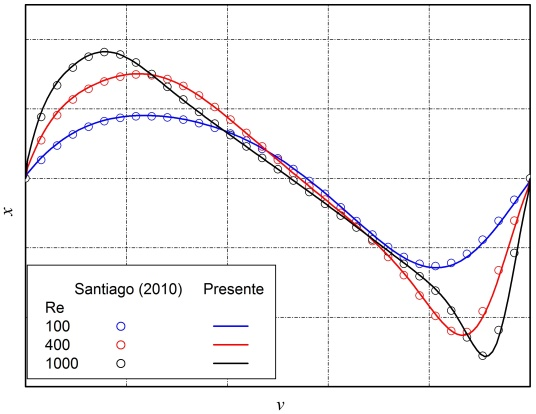
\includegraphics[width = \CaptionWidth]{grph-example}
\SourceOrNote{Autoria Própria (2024)}
\end{graph}

Em computação, é muito comum a utilização de fluxogramas, para documentar, estudar, planejar, melhorar e comunicar processos complexos por meio de diagramas claros e fáceis de entender. Um fluxograma é um diagrama que descreve um processo, sistema ou algoritmo de computador. O \Cref{fcht:ex-algorithm} é um dos vários exemplos deste tipo de ilustração que pode ser gerado ou editado na ferramenta \textit{online} \href{http://www.lucidchart.com/}{Lucidchart}, entre outras.

\begin{flowchart}[!htb]
\centering
\caption{Exemplo de fluxograma de algoritmo}%
\label{fcht:ex-algorithm}
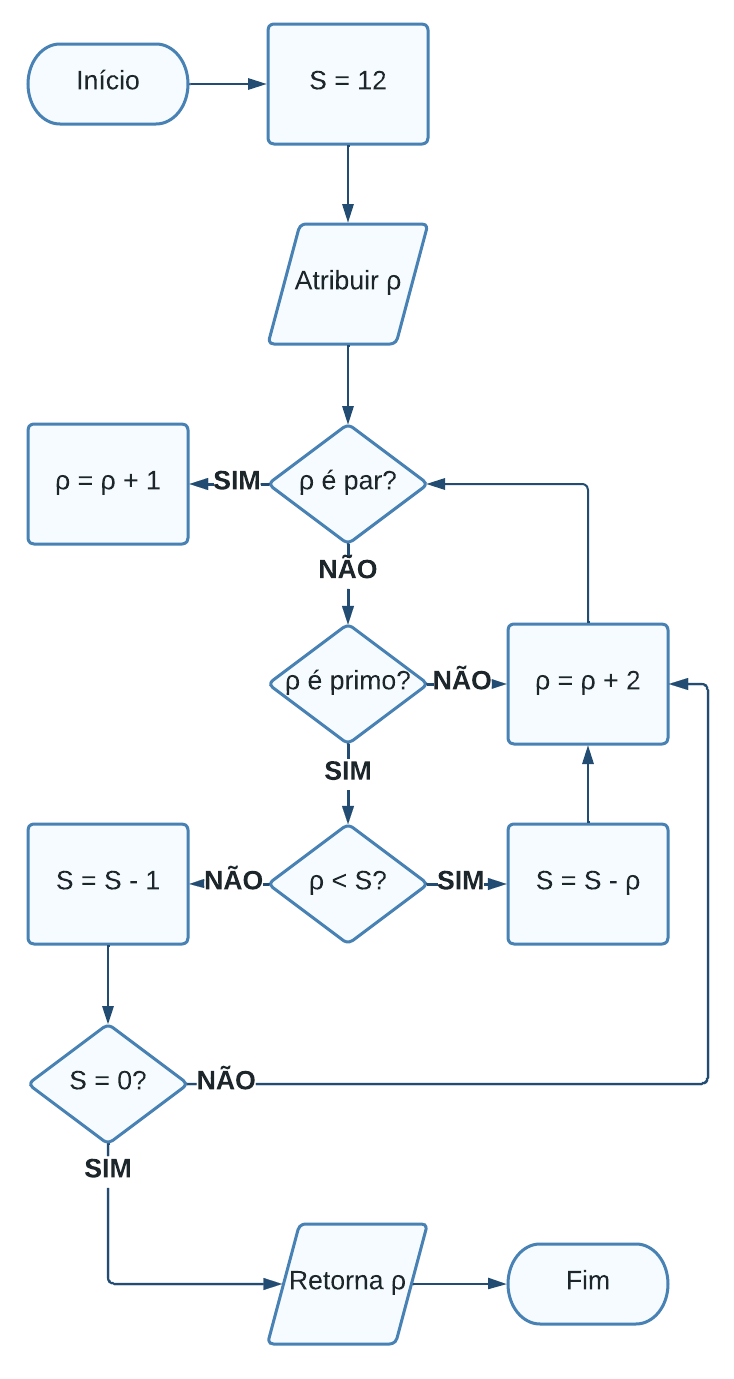
\includegraphics[scale=0.4]{fcht-ex-algorithm}
\SourceOrNote{Autoria Própria (2024)}
\end{flowchart}

O LaTeX tem uma biblioteca específica para utilizar imagens no documento. O pacote graphicx habilita um ambiente chamado figure, que permite que você insira imagens de uma forma simples no texto. A \Cref{fig:example-image-duck} é um exemplo deste tipo de ilustração.

\begin{figure}[!h]
\centering
\caption{Exemplo de figura}%
\label{fig:example-image-duck}
\includegraphics[scale=1.2]{example-image-duck}
\SourceOrNote{Autoria Própria (2024)}
\end{figure}

Caso seja necessário, você ainda poderá inserir fotografias, por meio do ambiente \textit{photograph}, conforme ilustrado na \Cref{phot:pg-campus}.

\begin{photograph}[!h]
\centering
\SetCaptionWidth{\ifbool{@LayoutA}{0.7}{0.72}\linewidth}
\caption{Fachada da Fatec de Registro}%
\label{phot:pg-campus}
\savebox0{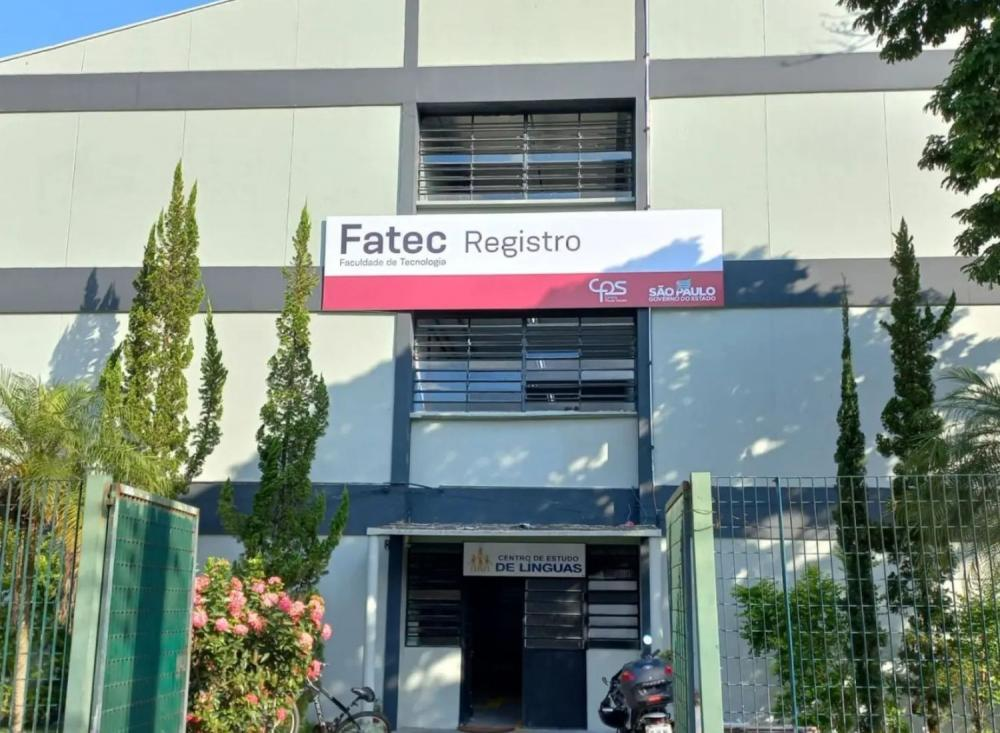
\includegraphics[width = \CaptionWidth]{Illustrations/fachada-fatec.jpg}}
\usebox0%
\SourceOrNote{Autoria Própria (2024)}
\end{photograph}

Outro elemento visual bastante utilizado na seção de Resultados são as tabelas, pois elas fornecem uma estrutura visualmente organizada para apresentar dados, tornando a leitura e a compreensão do conteúdo mais fácil para o leitor. As células, linhas e colunas ajudam a alinhar informações de maneira sistemática.

Para conjuntos de dados comparativos, as tabelas são particularmente úteis. Elas possibilitam a disposição lado a lado de informações relacionadas, facilitando a comparação direta entre diferentes elementos.

Tabelas e quadros devem estar centralizados e conter apenas dados imprescindíveis, evitando-se que sejam muito extensos, não repetindo dados já inseridos no texto, ou vice-versa. O formato de tabela pode ser observado na \Cref{tab:example}.

\begin{table}[!htb]
\centering
\SetCaptionWidth{0.5\linewidth}
\caption{Exemplo de tabela}%
\label{tab:example}
\begin{tabularx}{\CaptionWidth}{@{}XY@{}}
\toprule%
\rowcolor{TableColor}
\multicolumn{1}{Y}{\textcolor{white}{Idade}}           &
\multicolumn{1}{Y}{\textcolor{white}{Percentual (\%)}} \\
\midrule%
Até 20 anos     & 0  \\
De 21 a 30 anos & 10 \\
De 31 a 40 anos & 20 \\
De 41 a 50 anos & 30 \\
\bottomrule%
\end{tabularx}
\SourceOrNote{Adaptada de \textcite{Beltrano2021}}
\end{table}

No caso de quadros, deve ser seguida a estrutura demonstrada no \Cref{tfrm:typography}.
Caso os dados sejam inéditos e provenientes de uma pesquisa realizada pelos próprios autores do trabalho, essa especificação deve constar na fonte com o ano da pesquisa de campo.
Nesse caso, a fonte deve ser: Autoria Própria (2024).

\begin{tabframed}[!htb]
\centering
\caption{Tipografia das seções}%
\label{tfrm:typography}
\begin{tabularx}{\linewidth}{?{}p{20mm}|X|p{45mm}?{}}%% CHKTEX 44
\toprule%
\rowcolor{TableColor}
\multicolumn{1}{?{}c|}{\textcolor{white}{Seção}}   &
\multicolumn{1}{c|}{\textcolor{white}{Tipografia}} &
\multicolumn{1}{c?{}}{\textcolor{white}{Exemplo}}  \\
\midrule%
Primária                     &
Letras maiúsculas em negrito &
\textbf{1 SEÇÃO PRIMÁRIA}    \\
\midrule%
Secundária                    &
Letras maiúsculas sem negrito &
1.1 SEÇÃO SECUNDÁRIA          \\
\midrule%
Terciária                                                             &
Letra inicial de todas as palavras em maiúscula, sem negrito &
1.1.1 Seção Terciária                                                 \\
\midrule%
Quaternária                                                          &
Letra inicial da primeira palavra em maiúscula, sem negrito &
1.1.1.1 Seção quaternária                                            \\
\midrule%
Quinária                                                                          &
Letra inicial da primeira palavra em maiúscula, sem negrito e em itálico &
\textit{1.1.1.1.1 Seção quinária}                                                 \\
\bottomrule%
\end{tabularx}
\SourceOrNote{Autoria Própria (2024)}
\end{tabframed}

Quadros e tabelas podem ser inseridos neste documento usando os ambientes \texttt{tabframed} e \texttt{table}, respectivamente, conforme exemplos no arquivo-fonte deste modelo. A geração ou edição desses elementos visuais pode ser realizada por meio de ferramentas \textit{online}, tais como: \href{http://www.tablesgenerator.com/}{Tables Generator} e \href{http://www.latex-tables.com/}{Latex Tables Editor}, entre outras.

\subsection*{Equações}

Equações podem ser inseridas neste documento usando o ambiente  \texttt{equation}, como ilustrado na \Cref{eq:u}.

\begin{equation}%
\label{eq:u}
u = \beta \operatorname{sen} \left(\pi x\right) \frac{\left(e^{2x} - 1\right) \left(e^y - 1\right)}{\left(e^2 - 1\right) \left(e - 1\right)}
\end{equation}

Símbolos matemáticos (ou equações mais simples) podem ser inseridos ao longo do texto de um parágrafo usando o ambiente do Latex \texttt{math}. É possível ainda, a utilização de ferramentas onlines para a geração ou edição de equações, tais como: \href{http://formulasheet.com/}{Formula Sheet} e \href{http://www.tutorialspoint.com/latex_equation_editor.htm}{Latex Equation Editor}.



\section*{CONCLUSÃO}\label{sect:conclusao}

Apresente aqui as conclusões do seu trabalho, verifique se o objetivo foi cumprido, apresenta respostas para o problema da pesquisa, relate as limitações e as recomendações do estudo. Por fim, coloque sugestões para trabalhos futuros.

\printbibliography

%% Elementos pós-textuais (opcionais): Apêndice e Anexo
%Caso for utilizar, basta retirar o símbolo de % na frente do comando
%%%%% Elementos pós-textuais
%%
%% Glossário, apêndices, anexos e índice remissivo (opcionais).

%% Apêndices
\begin{Appendix}

\section{Título de Apêndice}%
\label{sect:apx-a1}

Exemplo de apêndice (\Cref{sect:apx-a1}) em uma seção de \nameref{sect:appendix}.

\subsection{Título de Seção Secundária de Apêndice}%
\label{ssect:apx-a2}

Exemplo de seção secundária de apêndice (\Cref{ssect:apx-a2}).

\subsubsection{Título de Seção Terciária de Apêndice}%
\label{sssect:apx-a3}

Exemplo de seção terciária de apêndice (\Cref{sssect:apx-a3}).

\paragraph{Título de seção quaternária de Apêndice}%
\label{prgh:apx-a4}

Exemplo de seção quaternária de apêndice (\Cref{prgh:apx-a4}).

\subparagraph{Título de seção quinária de Apêndice}%
\label{sprgh:apx-a5}

Exemplo de seção quinária de apêndice (\Cref{sprgh:apx-a5}).

\end{Appendix}

%% Anexos
\begin{Annex}

\section{Título de Anexo}%
\label{sect:anx-a1}

Exemplo de anexo (\Cref{sect:anx-a1}) em uma seção de \nameref{sect:annex}.

\subsection{Título de Seção Secundária de Anexo}%
\label{ssect:anx-a2}

Exemplo de seção secundária de anexo (\Cref{ssect:anx-a2}).

\subsubsection{Título de Seção Terciária de Anexo}%
\label{sssect:anx-a3}

Exemplo de seção terciária de anexo (\Cref{sssect:anx-a3}).

\paragraph{Título de seção quaternária de Anexo}%
\label{prgh:anx-a4}

Exemplo de seção quaternária de anexo (\Cref{prgh:anx-a4}).

\subparagraph{Título de seção quinária de Anexo}%
\label{sprgh:anx-a5}

Exemplo de seção quinária de anexo (\Cref{sprgh:anx-a5}).

\end{Annex}

%% Índice remissivo
\printindex%


%% Fim do documento
\end{document}